\documentclass[ignorenonframetext, professionalfonts, hyperref={pdftex, unicode}]{beamer}
%\usepackage{beamerthemesplit}

\geometry{paperwidth=140mm,paperheight=105mm}

%Hack to specify beamer folder https://tex.stackexchange.com/questions/275600/beamer-themes-on-custom-folder
\makeatletter
  \def\beamer@calltheme#1#2#3{%
    \def\beamer@themelist{#2}
    \@for\beamer@themename:=\beamer@themelist\do
    {\usepackage[{#1}]{\beamer@themelocation/#3\beamer@themename}}}

  \def\usefolder#1{
    \def\beamer@themelocation{#1}
  }
  \def\beamer@themelocation{}
\makeatother
%Packages to be included

\usepackage{graphicx}



\graphicspath{{./branding/}}
\usefolder{./branding}
\usetheme{Promwad}
%\usecolortheme{wolverine}


\usepackage[russian]{babel}
\usepackage[utf8]{inputenc}
\usepackage[T1]{fontenc}

%\usepackage[orientation=landscape, size=custom, width=16, height=9, scale=0.5]{beamerposter}

\usepackage{textcomp}


\usepackage{ulem}

\usepackage{verbatim}

\usepackage{ucs}


\usepackage{listings}
\lstloadlanguages{bash}

\lstset{escapechar=`,
	extendedchars=false,
	language=sh,
	frame=single,
	tabsize=2, 
	columns=fullflexible, 
%	basicstyle=\scriptsize,
	keywordstyle=\color{blue}, 
	commentstyle=\itshape\color{brown},
%	identifierstyle=\ttfamily, 
	stringstyle=\mdseries\color{green}, 
	showstringspaces=false, 
	numbers=none, 
%	numberstyle=\tiny, 
	breaklines=true, 
	inputencoding=utf8,
	keepspaces=true,
	morekeywords={u\_short, u\_char, u\_long, in\_addr}
	}

\definecolor{darkgreen}{cmyk}{0.7, 0, 1, 0.5}

\lstdefinelanguage{diff}
{
    morekeywords={+, -},
    sensitive=false,
    morecomment=[l]{//},
    morecomment=[s]{/*}{*/},
    morecomment=[l][\color{darkgreen}]{+},
    morecomment=[l][\color{red}]{-},
    morestring=[b]",
}

\author[Promwad]{{\bf Promwad}}

%\institution[EPAM]{EPAM}
%\logo{\includegraphics[width=1cm]{logo.png}}

\AtBeginSection[]{%
  \begin{frame}<beamer>
    \frametitle{}
    \tableofcontents[
        sectionstyle=show/shaded, hideallsubsections ]
  \end{frame}
  \addtocounter{framenumber}{-1}% If you don't want them to affect the slide number
}

\AtBeginSubsection[]{%
  \begin{frame}<beamer>
    \frametitle{}
    \tableofcontents[
        sectionstyle=show/hide,
        subsectionstyle=show/shaded/hide, ]
  \end{frame}
  \addtocounter{framenumber}{-1}% If you don't want them to affect the slide number
}


\title{Полезные сведения о компьютерной архитектуре}

\begin{document}

\begin{frame}
  \frametitle{}
\end{frame}

\section{Архитектура процессора}
\mode<all>{
\begin{frame}
 \frametitle{Классификация}
 \begin{itemize}
   \item Архитектура набора команд (Instruction set architecture)
   \item Микроархитектура
 \end{itemize}
\end{frame}
\subsection{Mикроархитектура}
\begin{frame}
 \frametitle{Микроархитектура}
 \textbf{Микроархитектура} -- определяет конкретную реализацию системы команд в железе. 

 \textbf{Важные элементы}
 \begin{itemize}
  \item Количество тактов на инструкцию
  \item Длина и структура конвейера
  \item Размер и структура кэшей
  \item Организация периферийных шин
 \end{itemize}
\end{frame}

\begin{frame}
  \frametitle{Пример: микроархитектура Intel Core}
  \includegraphics[height=6cm]{slides/processor_arch/Intel_Core2_arch.png}
\end{frame}
\subsection{Архитектура системы команд}
\begin{frame}
 \frametitle{Архитектура системы команд}
 \begin{center}
   {\bf\large Основные возможности}
 \end{center}
 \begin{itemize}
     \item Гарвардская/фон Неймановская
     \item RISC/CISC/VLIW/EPIC
     \item Разрядность (8/16/32/64)
     \item Число и типы регистров
     \item Максимальное число операндов (1,2,3,\dots) 
     \item Тип операндов (Регистр-регистр, Регистр-память, Память-память, Стековая машина)
     \item Кодировка инструкций (переменной длины, постоянной длины)
     \item Порядок байтов (старшего к младшему (big endian), младшего к старшему (little endian))
     \item Расширения
 \end{itemize}
\end{frame}

\begin{frame}
  \frametitle{Intel x86}
  \begin{itemize}
    \item фон Неймановская (модифицированная)
    \item CISC
    \item 16-64 бита 
    \item 8 специализированных регистров, 3-6 сегментных регистров, IP, 8 неспециализированных регистров, SIMD
    \item Max operands 2(3 for AVX)
    \item Регистр-память
    \item Переменной длины
    \item Little endian
    \item SSE, MMX, 3dNow
  \end{itemize}
\end{frame}

\begin{frame}
  \frametitle{ARM/ARMv7}
  \begin{itemize}
      \item фон Неймановская модифицированная
      \item RISC
      \item 16/32
      \item 7/15 неспециализированных регистров
      \item Регистр-регистр
      \item Фиксированная (32/16), Thumb-2 переменной длины
      \item Little/Big endian (mostly little)
      \item VFP, NEON, Jazelle,TrustZone
  \end{itemize}
\end{frame}

\begin{frame}
  \frametitle{MIPS}
  \begin{itemize}
      \item фон Неймановская модифицированая
      \item RISC
      \item 32/64
      \item 4-32 неспециализированных регистра
      \item Регистр-регистр
      \item Фиксированная(32)
      \item Big/Little endian
      \item MDMX, MIPS-3d
      \item задержка перехода (branch delay slot)
   \end{itemize}
\end{frame}
\subsection{Виртуальная адресация}
\begin{frame}
  \frametitle{Виртуальное адресное пространство}
  \begin{center}
    \includegraphics[height=6cm]{slides/processor_arch/Virtual_address_space_and_physical_address_space_relationship.png}
  \end{center}
\end{frame}
\begin{frame}
  \frametitle{Таблица страниц(page table):Intel PAE}
  \begin{center}
    \includegraphics[height=6cm]{slides/processor_arch/X86_Paging_PAE_2M.png}
  \end{center}
\end{frame}

\begin{frame}
  \frametitle{Таблица страниц: ARM}
  \begin{center}
    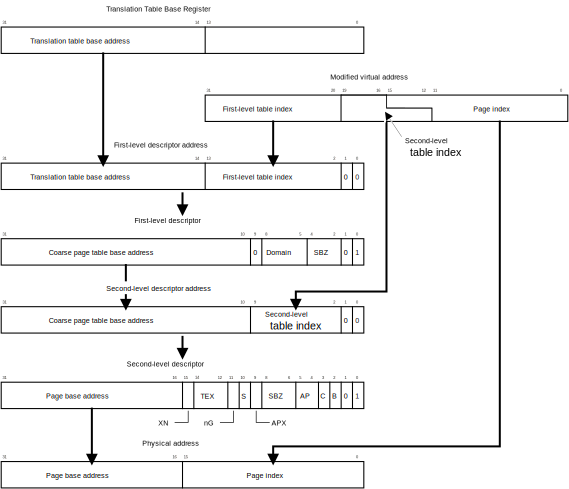
\includegraphics[height=6cm]{slides/processor_arch/large_page_table_walk_armv6_format.png}
  \end{center}
\end{frame}

\begin{frame}
  \frametitle{Буфер ассоциативной трансляции(TLB)}
  \begin{center}
    \includegraphics[height=6cm]{slides/processor_arch/Translation_Lookaside_Buffer.png}
  \end{center}
\end{frame}

}
\section{Периферийные устройства}
\mode<all>{\subsection{UART}
\begin{frame}
  \frametitle{UART(УАПП универсальный асинхронный приемопередатчик)}
  \begin{columns}
    \column{4cm}
    \includegraphics[width=4cm]{./slides/hardware_protocols/uart_bus.jpg}
    \column{4.5cm}
    \includegraphics[width=5cm]{./slides/hardware_protocols/UART_timing_diagram.png}
  \end{columns}
\end{frame}

\begin{frame}
  \frametitle{UART:свойства}
  \begin{columns}
    \column{4cm}
    \begin{center}
      {\bf\large Достоинства}
    \end{center}
    \begin{itemize}
       \item Отн. быстрый
       \item Мало проводов
    \end{itemize}
    \column{4cm}
    \begin{center}
      {\bf\large Недостатки}
    \end{center}
    \begin{itemize}
       \item Боится погрешности часов 
       \item Асинхронность менее надежна
       \item Peer2peer
    \end{itemize}
  \end{columns}
  \begin{center}
    {\bf\large Типичное применение}
  \end{center}
  Интерфейс отладки (консоль), GPS, модемы
\end{frame}
\subsection{I$^2$C}   
\begin{frame}
  \frametitle{I$^2$C}
  \begin{center}
    \includegraphics[height=3cm]{./slides/hardware_protocols/I2C.png}
    \vspace{0.3cm}

    \includegraphics[height=1.5cm]{./slides/hardware_protocols/600px-I2C_data_transfer.png}
  \end{center}
\end{frame}

\begin{frame}
  \frametitle{I$^2$C:свойства}
  \begin{columns}
    \column{4cm}
    \begin{center}
      {\bf\large Достоинства}
    \end{center}
    \begin{itemize}
       \item Много периферии на три провода
       \item Синхронный
    \end{itemize}
    \column{4cm}
    \begin{center}
      {\bf\large Недостатки}
    \end{center}
    \begin{itemize}
       \item Отн. медленный
       \item Сложный
    \end{itemize}
  \end{columns}
  \begin{center}
    {\bf\large Типичное применение}
  \end{center}
  Взаимодействие с датчиками: гироскоп, термометр, АЦП, магнетометр; часть протокола HDMI
\end{frame}
\subsection{SPI}
\begin{frame}
  \frametitle{SPI}
  \begin{columns}
    \column{4cm}
    \includegraphics[width=4cm]{./slides/hardware_protocols/SPI_three_slaves.png}
    \column{4cm}
    \includegraphics[width=4cm]{./slides/hardware_protocols/SPI_8-bit_circular_transfer.png}
  \end{columns}
  \begin{center}
    \includegraphics[height=3cm]{./slides/hardware_protocols/SPI_timing_diagram2.png}
  \end{center}
\end{frame}

\begin{frame}
  \frametitle{SPI:свойства}
  \begin{columns}
    \column{4cm}
    \begin{center}
      {\bf\large Достоинства}
    \end{center}
    \begin{itemize}
       \item Быстрый
       \item Синхронный
       \item Простой
    \end{itemize}
    \column{4cm}
    \begin{center}
      {\bf\large Недостатки}
    \end{center}
    \begin{itemize}
       \item Много проводов (SS)
    \end{itemize}
  \end{columns}
  \begin{center}
    {\bf\large Типичное применение}
  \end{center}
  Взаимодействие с датчиками, взаимодействие с flash памятью, взаимодействие с некоторыми ethernet контроллерами
\end{frame}
\subsection{GPIO}
\begin{frame}
  \frametitle{GPIO}
  \textbf{GPIO(Интерфейс ввода/вывода общего назначения)} -- универсальный интерфейс, в котором установка выводов процессора в логические состояния полностью контролируется программно.
  

  \begin{columns}
    \column{4cm}
    \begin{center}
      {\bf\large Достоинства}
    \end{center}
    \begin{itemize}
       \item Наиболее универсальный
    \end{itemize}
    \column{4cm}
    \begin{center}
      {\bf\large Недостатки}
    \end{center}
    \begin{itemize}
       \item Тратятся дорогие циклы процессора
    \end{itemize}
  \end{columns}
  \begin{center}
    {\bf\large Типичное применение}
  \end{center}
  Индикаторы, включатели/выключатели, прием данных от кнопок, реализация отсутствующих железных интерфейсов

\end{frame}
\subsection{USB}
\begin{frame}
  \frametitle{USB}
  \begin{columns}
    \column{4cm}
    \begin{center}
      {\bf\large Достоинства}
    \end{center}
    \begin{itemize}
       \item Универсальный
       \item Быстрый
    \end{itemize}
    \column{4cm}
    \begin{center}
      {\bf\large Недостатки}
    \end{center}
    \begin{itemize}
       \item Дорогие контроллеры
       \item Очень сложный
    \end{itemize}
  \end{columns}
  \begin{center}
    {\bf\large Типичное применение}
  \end{center}
  Взаимодействие с пользователем (USB HID), взаимодействие с flash хранилищами (USB Storage), передача медиаданных (USB UVC, звуковые карты), 
\end{frame}
}
\section{Разработка для железа}
\subsection{Что на входе}
\begin{frame}
  \frametitle{Входные данные}
  \begin{itemize}
      \item В идеале
        \begin{itemize}
            \item Загрузчик, сконфигурированный под плату
            \item Ядро, сконфигурированное под  плату
            \item Device Tree 
        \end{itemize}
      \item Минимально необходимая информация
        \begin{itemize}
          \item Документация(datasheet) на процессор или SoC
          \item Документация на все устройства подключенные по внешним шинам
          \item Схема соединений
        \end{itemize}
  \end{itemize}
\end{frame}
\begin{frame}
  \frametitle{Что содержится в документации на SoC/процессор/внешние устройства}
  \begin{itemize}
      \item Memory mapping
      \item Hardware controlling registers, описание функций
      \item Архитектура прерываний, используемые прерывания
  \end{itemize}
\end{frame}
\begin{frame}
  \frametitle{Типичные задачи при освоении новой платы}
  \begin{itemize}
      \item Портирование u-boot
      \item Портирование deviceTree
      \item Написание модулей ядра (драйверов устройств)
  \end{itemize}
\end{frame}
\subsection{Представление информации об архитектуре для ядра (devicetree)}
\begin{frame}
  \frametitle{DeviceTree: что это такое?}
\textbf{DeviceTree} -- структура данных, содержащая информацию о конфигурации конкретной платы. 

\vspace{1cm}

Существует в двух модификациях -- человекочитаемая (файлы \texttt{*.dts}) и машиночитаемая (файлы \texttt{*.dtb})

\vspace{1cm}

Бинарный файл devicetree загружается в память одновременно с ядром, и используется ядром для подбора драйверов и загрузки параметров драйверов.
\end{frame}

\begin{frame}
  \frametitle{Пример devicetree файла}
\end{frame}

\begin{frame}
  \frametitle{DeviceTree: Зачем это нужно?}
  \begin{itemize}
     \item Меньше вариантов сборки ядра
     \item Возможность поддерживать новые платы без пересборки ядра
     \item Меньше коммитов в драйвера ядра 
     \item Приспособлены для автоматизации
  \end{itemize}
\end{frame}
\begin{frame}
  \frametitle{Родственные технологии}
  \begin{itemize}
      \item Внутриядерные структуры данных с описанием архитектуры платы (/arch/arm/mach-*) 
      \item UEFI
      \item ACPI (i386 only)
      \item OpenFirmware (PowerPC, Solaris) прямой предок
  \end{itemize}
\end{frame}

\begin{frame}
  \frametitle{Наиболее интересные параметры в описании устройства}
  \begin{itemize}
    \item \texttt{compatible} -- строка, определяет выбор драйвера
    \item \texttt{status} -- строка, используется ли устройство \texttt{"ok"}/\texttt{"disabled"}
  \end{itemize}
\end{frame}

\begin{frame}
  \frametitle{Наиболее важные разделы DeviceTree}
  \begin{itemize}
    \item \textbf{cpus} Процессоры
    \item \textbf{memory} Структура памяти
    \item \textbf{aliases}
    \item \textbf{choosen} Параметры загрузки
  \end{itemize}
\end{frame}

\begin{frame}[fragile]
  \frametitle{Оверлеи пример}
\begin{lstlisting}
// Enable the i2s interface
/dts-v1/;
/plugin/;

/ {
    compatible = "brcm,bcm2708";

    fragment@0 {
        target = <&i2s>;
        __overlay__ {
            status = "okay";
        };
    };
};
\end{lstlisting}
\end{frame}
\begin{frame}[fragile]
 \frametitle{Оверлеи}
\begin{lstlisting}[language=bash]
dtc -@ -I dts -O dtb -o patch.dtbo overlay.dts
dtoverlay patch.dtbo
dtoverlay -r patch.dtbo
\end{lstlisting}
\end{frame}
\end{document}
